\section{Sunday, 4 November 2018}

\subsection{Interpreting results}
\subsubsection{Accelerometer}
\begin{itemize}
\item In the first group we can conclude supposing that the person is stand up because the axis Y has got the maximum value.
\item The second and the third group we can suppose that the person is walking because the values isn't so clearly. 
\item The fourth group has got values near to 0 and because that we can suppose the mobile phone is in repose.
\end{itemize}
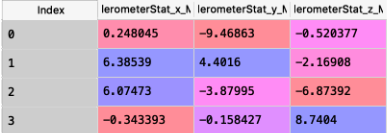
\includegraphics{images/CentroidsMean_Accelerometer}

\subsubsection{Gyroscope}
\begin{itemize}
\item In the first and third group with the values we can't see anything clear. We can suppose that the person is walking.
\item In the second group we can see how the mobile is in repose.

\end{itemize}
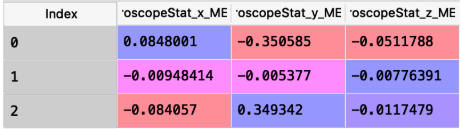
\includegraphics{images/CentroidsMean_Gyroscope}

\subsubsection{Outliers}
In the accelerometer outliers hasn't relationship with each other but we can see that this values are near with other outliers, so it's possible that the person had done something stranger.\\

On the other hand, in the gyroscope outliers is the same case that accelerometer, but we can see the all outliers values are near to 0. It's all we can say because we haven't got more data
